\documentclass[fleqn]{article}
\usepackage[x11names, rgb]{xcolor}
\usepackage[utf8]{inputenc}
\usepackage{tikz}
\usepackage{amsmath}
\usepackage{geometry}
\usepackage{fancyhdr}
\usepackage{amsmath,amsthm,amssymb}
\usepackage{graphicx}
\usepackage{hyperref}
\usepackage{lipsum}
\usepackage{ulem}
\usepackage{comment}
\usepackage{enumerate}
\usepackage{titlesec}
\usepackage{boolexpr,pdftexcmds,trace}
\usepackage{pgfplotstable}
\usepackage{standalone}
\makeatletter

\graphicspath{{./screenshots/}}
\DeclareGraphicsExtensions{.png}   

\usetikzlibrary{snakes,arrows,shapes}
\newwrite\dotfile

\begingroup
  \catcode`\[ = 1\relax
  \catcode`\] = 2\relax
  \catcode`\{ = 12\relax
  \catcode`\} = 12 \relax
  \gdef\OpenBrace[{]
  \gdef\CloseBrace[}]
\endgroup

% custom commands
\newcommand{\leadingzero}[1]{\ifnum #1<10 0#1\else#1\fi}
\newcommand{\gerdate}[3]{\leadingzero{#1}.\leadingzero{#2}.\leadingzero{#3}}
\newcommand{\gertoday}{\gerdate{\the\day}{\the\month}{\the\year}}
\newcommand*{\bfrac}[2]{\genfrac{}{}{0pt}{}{#1}{#2}}
\newcommand{\R}{\mathbb{R}}
\newcommand{\N}{\mathbb{N}}
\newcommand{\Q}{\mathbb{Q}}
\newcommand{\Z}{\mathbb{Z}}
\newcommand{\dotarrow}[0]{}

\newenvironment{graphviz}[1]%
{%
\switch
\case{\pdf@strcmp{#1}{graph}}
    \renewcommand{\dotarrow}[0]{--}
\case{\pdf@strcmp{#1}{strict graph}}
    \renewcommand{\dotarrow}[0]{--}
\case{\pdf@strcmp{#1}{digraph}}
    \renewcommand{\dotarrow}[0]{->}
\case{\pdf@strcmp{#1}{strict digraph}}
    \renewcommand{\dotarrow}[0]{->}
\endswitch

\immediate\openout\dotfile=tmp.dot%
\newcommand{\node}[2]{%
\immediate\write\dotfile{##1 \dotarrow \OpenBrace##2\CloseBrace}%
}%
%
\immediate\write\dotfile{#1 \OpenBrace}
}%
{\immediate\write\dotfile{\CloseBrace}%
\immediate\closeout\dotfile%
\immediate\write18{dot2tex --figonly tmp.dot > tmp.tex}%
\input{tmp.tex}%
}

\setcounter{section}{0}
\setcounter{subsection}{0}
\pagestyle{fancy}

\lhead{Tobias Knöppler, Klaus Ziegert}
\chead{}
\rhead{\gertoday}
\lfoot{}
\cfoot{\thepage}
\rfoot{}
%\setlength{\mathindent}{0pt}

% document specific settings
%\renewcommand{\thesection}{}
\renewcommand{\thesubsection}{\arabic{section}. \alph{subsection})}
\renewcommand{\thesubsubsection}{\roman{subsubsection})}
\titleformat{\subsubsection}[runin]{\normalfont\normalsize\bfseries}{\thesubsubsection}{1em}{}

\title{Visualisierung}
\begin{document}
\section{Anwendungsbeispiel}
\begin{center}
mpirun -np 8 circle 20\\
\begin{tabular}{|l|l|}            \hline\hline
Before & After\\
rank 0: 22 & rank 0: 1\\ 
rank 0: 12 & rank 0: 5\\
rank 0: 11 & rank 0: 7\\
rank 1: 1 & rank 1: 13\\
rank 1: 5 & rank 1: 6\\
rank 1: 7 & rank 1: 23\\
rank 2: 13 & rank 2: 14\\
rank 2: 6 & rank 2: 6\\
rank 2: 23 & rank 2: 3\\
rank 3: 14 & rank 3: 1\\
rank 3: 6 & rank 3: 14\\
rank 3: 3 & rank 4: 20\\
rank 4: 1 & rank 4: 5\\
rank 4: 14 & rank 5: 1\\
rank 5: 20 & rank 5: 11\\
rank 5: 5 & rank 6: 11\\
rank 6: 1 & rank 6: 5\\
rank 6: 11 & rank 7: 22\\
rank 7: 11 & rank 7: 12\\
rank 7: 5 & rank 7: 11\\
\hline
\end{tabular}
\end{center}
\section{Visualisierung}
Die folgende Farbkodierung gilt für alle Screenshots:\\
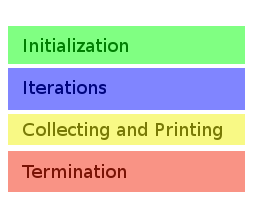
\includegraphics[scale=0.4]{caption}

\subsection{}%subsection name}\label{label}
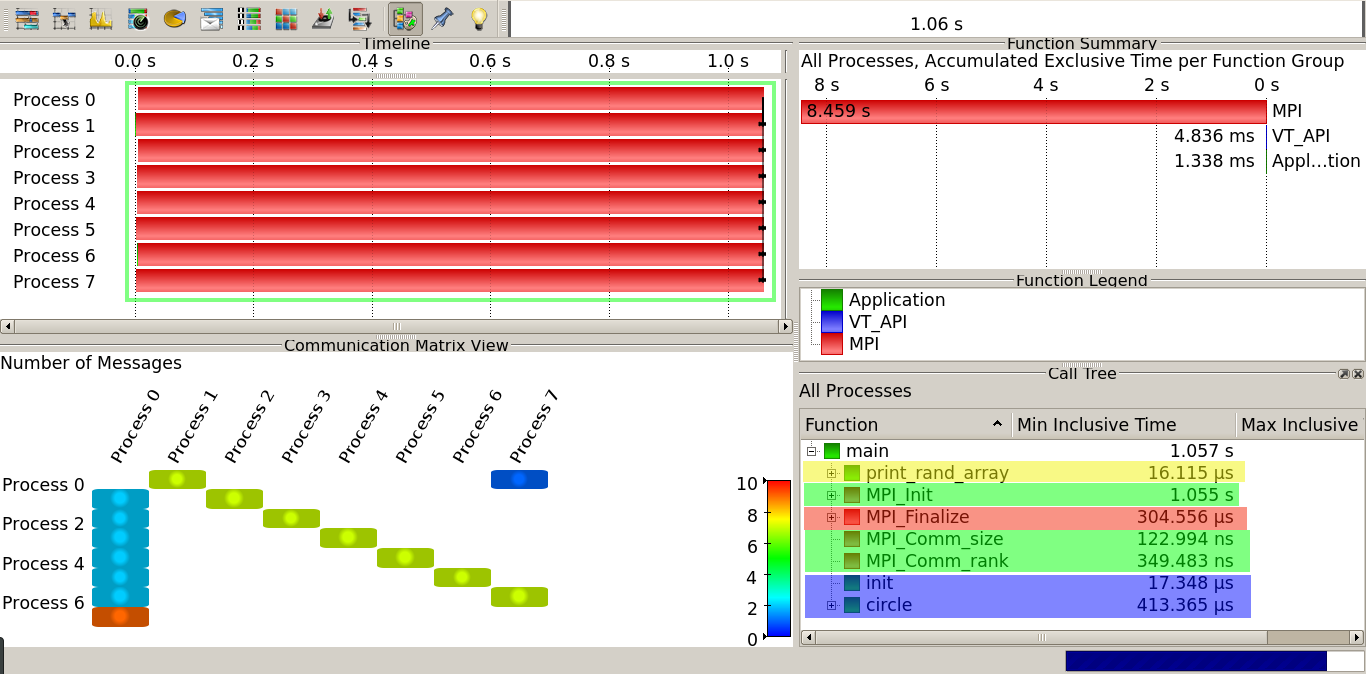
\includegraphics[width=\textwidth]{vampir1}

\subsection{}%subsection name}\label{label}
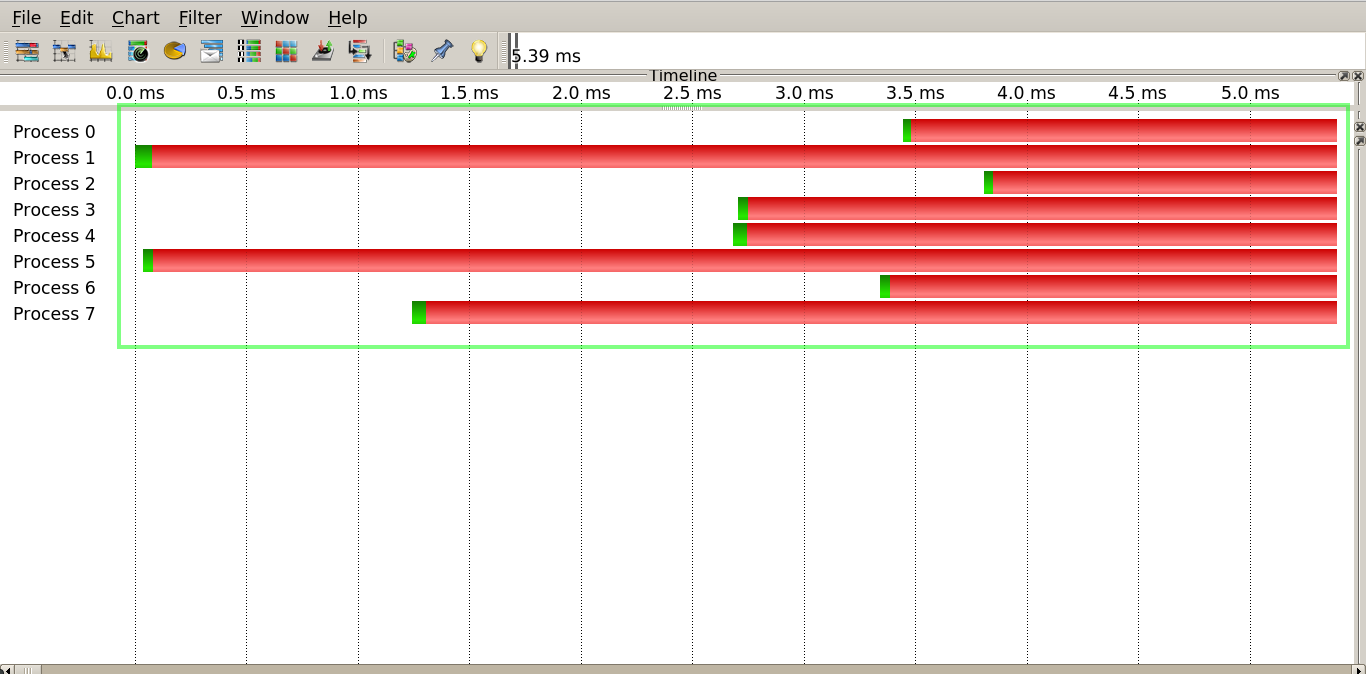
\includegraphics[width=\textwidth]{vampir2}

\subsection{}%subsection name}\label{label}
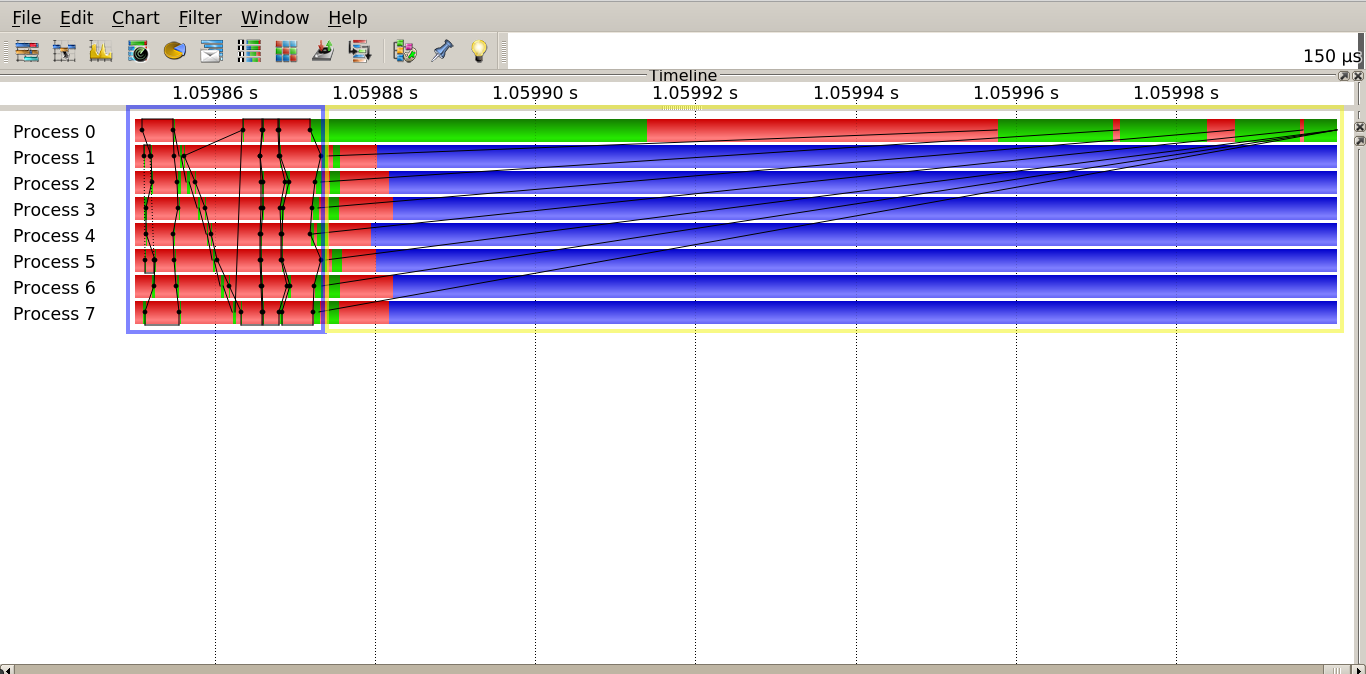
\includegraphics[width=\textwidth]{vampir3}

\subsection{}%subsection name}\label{label}

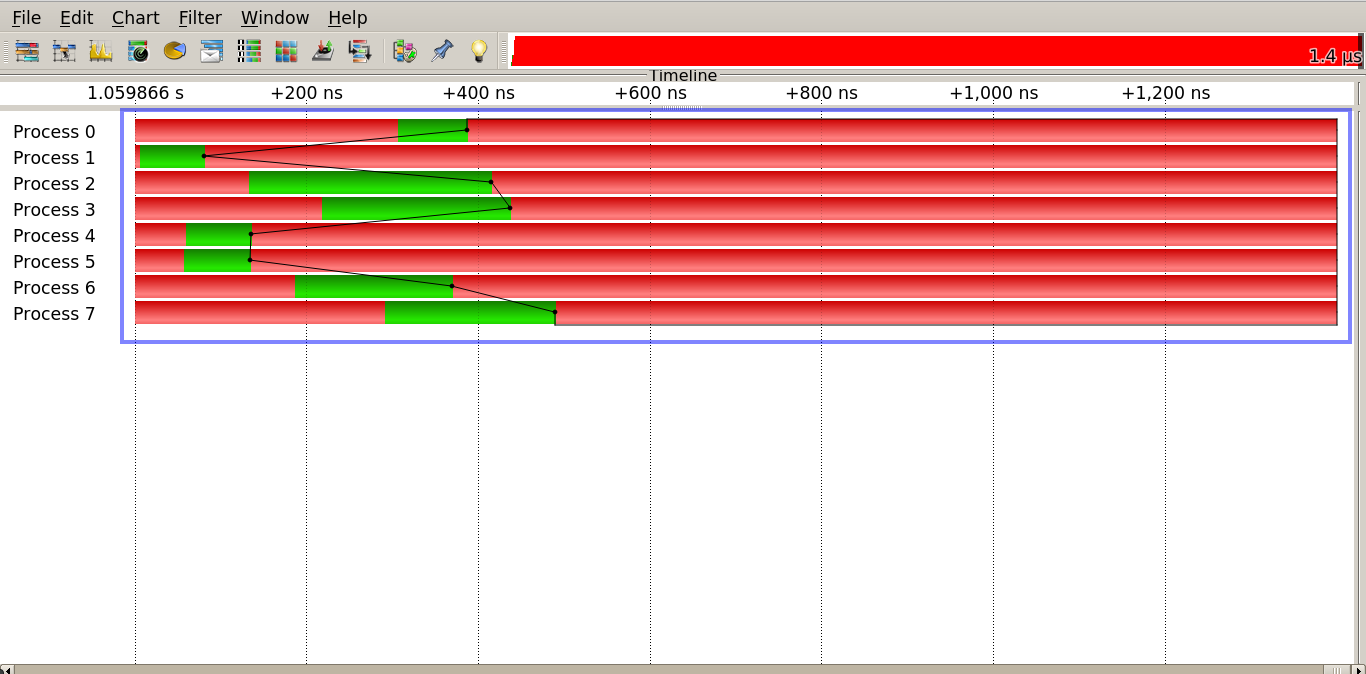
\includegraphics[width=\textwidth]{vampir4}



\end{document}
